\section{SAD}
\subsection{Analysephase}
\begin{frame} 
  \frametitle{Analyse} 
  Um die Anforderung \textbf{``Suchfunktion''} umsetzen zu können, müssen im Vorfeld einigen Fragen geklärt werden. 
   \begin{enumerate}
   \item Wie kann auf die Daten zugegriffen werden?
   \item Wie kann eine Autovervollständigung performant implementiert werden?
   \item Welche Technologien können verwendet werden?
   \item Welche Daten müssen geschützt werden?
   \item Wie kann die Suchfunktion intelligent gestaltet werden um die User 
   Experience zu erhöhen?
  \end{enumerate}
\end{frame}

\begin{frame} 
  \frametitle{Systemkontext}
  \begin{figure}[htbp]
\centering
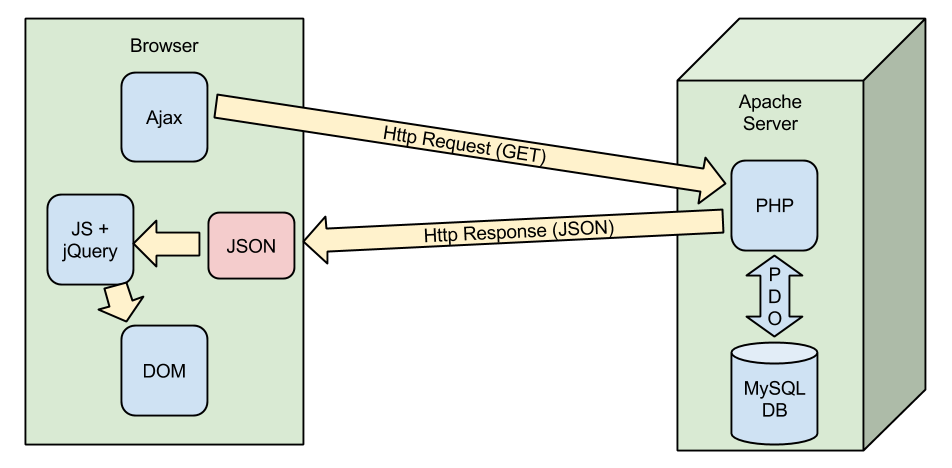
\includegraphics[width=1.0\textwidth]{./chapters/SAD_dynAccess.png}
\caption{Ablauf eines dynamischen Zugriffs}
\label{fig:SAD_dynAccess}
\end{figure}
\end{frame}

\begin{frame} 
  \frametitle{Verwendbare Technologien}
  \begin{block}{Java Script}
    Ausführen dynamischer Aktionen im Browser des Nutzers
  \end{block}
  \begin{block}{jQuery und Ajax}
    Umfangreiche Bibliothek für Java Script
  \end{block}
  \begin{block}{PHP}
    Serverseitige Datenverarbeitung sowie Datenbankzugriff
  \end{block}
  \begin{block}{PDO}
    Abstraktionsebene für Datenbankzugriffe
  \end{block}
\end{frame}

\begin{frame} 
  \frametitle{Performance und Datenschutz}
  \highlighton{Performance}
  \begin{itemize}
    \item Dynamische Anfragen über Ajax
    \item Wenig Datenbankzugriffe
    \item Datenbankoptimierung
  \end{itemize} 
  \highlighton{Datenschutz}
  \begin{itemize}
    \item Request frühzeitig in Java Script und PHP validieren 
    \item Datenbankabfragen auf SQL-Injection prüfen
    \item Vertrauliche Daten über Nutzerrechte der Datenbank schützen
  \end{itemize}
\end{frame}

\begin{frame}
  \frametitle{User Experience}
  \textbf{Die Suchfunktion} soll den Nutzer der Seite unterstützen und intelligent die 
  gewünschten Ergebnisse präsentieren. \newline \newline
  \highlighton{Features:}
  \begin{itemize}
    \item Automatische Vorschläge bei einer Eingabe
    \item Mögliche Ausgaben:
    \begin{itemize}
      \item Wohnort eines Tutors
      \item Benutzername eines Tutors (wenn Nutzer eingeloggt ist)
      \item Unterrichtsfach
    \end{itemize}
    \item Automatische Weiterleitung des Nutzers auf passende Seite
  \end{itemize} 
 \end{frame}
 
 \begin{frame}
   \frametitle{Suchfunktion}
    \textbf{Beispiele:} \newline
  \highlighton{Auswahl:} Wohnort $\rightarrow$ Anzeige aller Tutoren an diesem Ort \newline
   \highlighton{Auswahl:} Tutor $\rightarrow$ Anzeige des Tutorprofils \newline
   \highlighton{Auswahl:} Fach $\rightarrow$ Anzeige aller Tutoren die dieses Fach unterrichten \newline
 \end{frame}
 